% =====================================================================
%  Urban Track  |  Trust layer for urban development
%  Client presentation - built with Beamer (metropolis) + XeLaTeX
%  Accurately reflects the current state of the delivered application.
% =====================================================================
\documentclass[aspectratio=169, 10pt]{beamer}

\usepackage{fontspec}
\usepackage{xcolor}
\usepackage{graphicx}
\usepackage{tikz}
\usetikzlibrary{shapes.geometric, arrows.meta, positioning, calc, decorations.pathreplacing}
\usepackage[most]{tcolorbox}
\usepackage{pifont}
\usepackage{booktabs}
\usepackage{array}

\tcbset{before skip=0pt, after skip=0pt}

% ---------------------------------------------------------------------
% Fonts
% ---------------------------------------------------------------------
\setsansfont{Lato}
\setmonofont{DejaVu Sans Mono}

% ---------------------------------------------------------------------
% Palette - "Urban" identity
% ---------------------------------------------------------------------
\definecolor{utnavy}{HTML}{16324F}
\definecolor{utteal}{HTML}{0F766E}
\definecolor{utamber}{HTML}{D97706}
\definecolor{utgreen}{HTML}{15803D}
\definecolor{utred}{HTML}{B91C1C}
\definecolor{utgray}{HTML}{5B6B7C}
\definecolor{utlight}{HTML}{F1F5F9}
\definecolor{utcream}{HTML}{FDF6EC}

\usetheme{metropolis}

% Metropolis palette override
\setbeamercolor{palette primary}{bg=utnavy, fg=white}
\setbeamercolor{palette secondary}{bg=utteal, fg=white}
\setbeamercolor{title separator}{fg=utteal}
\setbeamercolor{progress bar}{fg=utamber}
\setbeamercolor{frametitle}{bg=utnavy, fg=white}
\setbeamercolor{section title}{bg=utnavy, fg=white}
\setbeamercolor{normal text}{fg=utnavy}
\setbeamercolor{structure}{fg=utteal}
\setbeamercolor{block title}{fg=white, bg=utnavy}
\setbeamercolor{block body}{fg=utnavy, bg=utlight}
\setbeamercolor{block title alerted}{fg=white, bg=utred}
\setbeamercolor{block body alerted}{fg=utnavy, bg=utlight}
\setbeamercolor{block title example}{fg=white, bg=utteal}
\setbeamercolor{block body example}{fg=utnavy, bg=utlight}

\metroset{block=fill, sectionpage=none, numbering=fraction}

% ---------------------------------------------------------------------
% Helper commands
% ---------------------------------------------------------------------
\newcommand{\chip}[2]{%
  \tikz[baseline=-0.6ex]{\node[rounded corners=2pt, inner sep=2.5pt, fill=#1, text=white,
    font=\scriptsize\bfseries]{#2};}%
}

\newcommand{\done}{\chip{utgreen}{LIVE}}
\newcommand{\partialc}{\chip{utamber}{PARTIAL}}
\newcommand{\togo}{\chip{utred}{NEXT}}

\newcommand{\keypoint}[1]{%
  \begin{tcolorbox}[enhanced, colback=utlight, colframe=utteal,
    boxrule=0pt, leftrule=3pt, arc=2pt, boxsep=4pt, left=6pt, right=6pt, top=4pt, bottom=4pt]
    \color{utnavy}#1
  \end{tcolorbox}%
}

\newcommand{\cstat}[3]{%
  \begin{tabular}{@{}p{2.05cm}@{}}
    \centering{\fontsize{24}{26}\selectfont\color{#2}\textbf{#1}}\\[2pt]
    \centering{\scriptsize\color{utgray}#3}
  \end{tabular}%
}

\newcommand{\shotscreen}[3][0.40\paperheight]{%
  \begin{tcolorbox}[enhanced, colback=white, colframe=utnavy!70, boxrule=0.8pt,
    arc=3pt, before skip=0pt, after skip=0pt, boxsep=4pt, width=\linewidth]
    \includegraphics[width=\linewidth,height=#1,keepaspectratio]{img/#2}
  \end{tcolorbox}%
  {\centering\scriptsize\color{utgray}#3\par}%
}

\setlength{\leftmargini}{0pt}
\setlength{\parskip}{4pt}

% =====================================================================
\title{Urban Track}
\subtitle{The trust layer of urban development --- cross-confirmed experience, permanent professional identity, and certified CVs}
\date{August 2026}

\begin{document}

% ---------------------------------------------------------------------
% 1. TITLE
% ---------------------------------------------------------------------
{
\setbeamercolor{background canvas}{bg=utnavy}
\begin{frame}[plain]
  \centering
  \vspace*{0.55cm}
  {\color{utamber}\footnotesize\bfseries URBAN TRACK SYSTEM}\\[6pt]
  {\color{white}\Huge\bfseries Trust layer of urban development}\\[12pt]
  {\color{utlight}\large Cross-confirmed experience, permanent professional identity,\\[2pt]
  and certified CVs for urban experts}\\[22pt]
  \begin{tcolorbox}[enhanced, colback=utteal, colframe=utteal,
    boxrule=0pt, arc=4pt, width=0.62\textwidth, center, boxsep=8pt]
    \color{white}\small\bfseries Client Presentation --- August 2026
  \end{tcolorbox}
  \vspace{0.35cm}
  {\color{utlight}\footnotesize Python (Django) \textbullet\ Tailwind CSS \textbullet\ PostgreSQL-ready \textbullet\ Trust \& certification}
  \vspace{0.25cm}
\end{frame}
}

% ---------------------------------------------------------------------
% 2. AGENDA
% ---------------------------------------------------------------------
\section{Agenda}

\begin{frame}{Agenda}
  \begin{columns}[T]
    \begin{column}{0.52\textwidth}
      \begin{itemize}
        \item \textbf{Why we built it} --- the problem behind Urban Track
        \item The solution in a nutshell
        \item \textbf{What's live today} --- real modules \& screens
        \item How trust gets certified
      \end{itemize}
    \end{column}
    \begin{column}{0.48\textwidth}
      \begin{itemize}
        \item Project portfolios, galleries \& reports
        \item Branded email notifications
        \item \textbf{Status} --- everything is built; ready for migration to the cloud
      \end{itemize}
    \end{column}
  \end{columns}
  \vspace{0.5cm}
  \keypoint{\textbf{One message in a nutshell:} the platform works today --- and it's built on verifiable trust, not on claims taken at face value.}
\end{frame}

% =====================================================================
% 3. VISION
% =====================================================================
\section{Project Vision}

\begin{frame}{The problem we set out to fix}
  \begin{columns}[T]
    \begin{column}{0.48\textwidth}
      \textbf{Working in urban development in Africa is held back by a lack of trust:}
      \vspace{4pt}
      \begin{itemize}
        \item \textbf{CVs that are hard to believe} --- no easy way to check what an expert really did; references rarely get followed up.
        \item \textbf{Credit that gets lost} --- big firms take the credit while the individuals who actually did the work stay invisible.
        \item \textbf{Data that stays siloed} --- agencies (World Bank, EU, AFD) don't share their records, so finding the right person is guesswork.
      \end{itemize}
    \end{column}
    \begin{column}{0.52\textwidth}
      \begin{tcolorbox}[enhanced, colback=utlight, colframe=utnavy, boxrule=0pt,
        leftrule=4pt, arc=2pt, boxsep=8pt]
        {\color{utnavy}\textbf{What that costs people:}}\\[2pt]
        \begin{itemize}
          \item Hours lost searching for qualified consultants
          \item Hiring mistakes and expertise that can't be verified
          \item Talented professionals who never get the recognition they earned
        \end{itemize}
      \end{tcolorbox}
      \vspace{4pt}
      \keypoint{\textbf{Our goal:} bring clarity, transparency and trust to urban expertise across Africa.}
    \end{column}
  \end{columns}
\end{frame}

\begin{frame}{How trust gets built}
  \begin{columns}[T]
    \begin{column}{0.33\textwidth}
      \begin{tcolorbox}[enhanced, colback=utnavy, colframe=utnavy, arc=3pt,
        boxsep=10pt, top=12pt, bottom=12pt, middle=10pt]
        \centering\color{utamber}\bfseries 1. Identity
        \vspace{4pt}
        {\color{white}\small Every expert gets a permanent \texttt{OX-XXXXXX} number that stays with them for life.}
      \end{tcolorbox}
    \end{column}
    \begin{column}{0.33\textwidth}
      \begin{tcolorbox}[enhanced, colback=utteal, colframe=utteal, arc=3pt,
        boxsep=10pt, top=12pt, bottom=12pt, middle=10pt]
        \centering\color{white}\bfseries 2. Cross-checking
        \vspace{4pt}
        {\color{white}\small Nothing gets certified unless a second party confirms it, by email, first.}
      \end{tcolorbox}
    \end{column}
    \begin{column}{0.33\textwidth}
      \begin{tcolorbox}[enhanced, colback=utamber, colframe=utamber, arc=3pt,
        boxsep=10pt, top=12pt, bottom=12pt, middle=10pt]
        \centering\color{utnavy}\bfseries 3. Trust score
        \vspace{4pt}
        {\color{utnavy}\small Confirmed work is weighted by role into one transparent, auditable score.}
      \end{tcolorbox}
    \end{column}
  \end{columns}
  \vspace{0.35cm}
  \begin{center}
  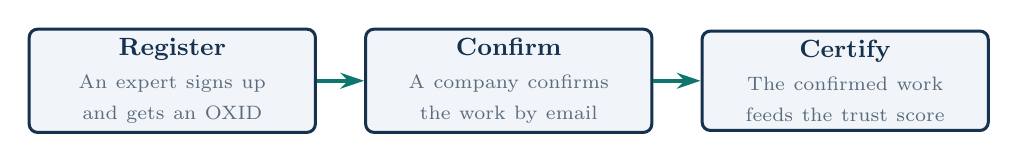
\begin{tikzpicture}[
    font=\small,
    node distance=0.4cm and 0.6cm,
    box/.style={rounded corners=3pt, draw, line width=1.1pt, minimum height=8mm, align=center,
      fill=utlight, text=utnavy, draw=utnavy, text width=3.4cm},
    arr/.style={-{Stealth[length=3mm, width=2mm]}, line width=1.4pt, draw=utteal}
  ]
    \node[box] (a) {\textbf{Register}\\[1pt]\scriptsize\color{utgray}An expert signs up and gets an OXID};
    \node[box, right=of a] (b) {\textbf{Confirm}\\[1pt]\scriptsize\color{utgray}A company confirms the work by email};
    \node[box, right=of b] (c) {\textbf{Certify}\\[1pt]\scriptsize\color{utgray}The confirmed work feeds the trust score};
    \draw[arr] (a) -- (b);
    \draw[arr] (b) -- (c);
  \end{tikzpicture}
  \end{center}
  \vspace{0.15cm}
  \centering\small\color{utgray}\emph{Identity first, then cross-confirmation, then certification --- nothing is taken at face value.}
\end{frame}

% =====================================================================
% 4. WHAT WE BUILT TODAY
% =====================================================================
\section{What Is Delivered Today}

\begin{frame}{Delivery at a glance}
  \begin{center}
  \cstat{10}{utteal}{data models}
  \hspace{2pt}
  \cstat{36}{utnavy}{URL routes}
  \hspace{2pt}
  \cstat{51}{utamber}{templates}
  \hspace{2pt}
  \cstat{6}{utgray}{application modules}
  \hspace{2pt}
  \cstat{183}{utteal}{automated tests}
  \hspace{2pt}
  \cstat{100\%}{utgreen}{core features live}
  \end{center}

  \vspace{0.15cm}
  \keypoint{\textbf{It all works end-to-end today ---} from sign-up to a permanent OXID, cross-confirmed trust scores, project galleries, certified CVs and a working job marketplace.}

  \vspace{0.12cm}
  \begin{center}
  
\begin{tikzpicture}[
    font=\small,
    box/.style={rounded corners=4pt, minimum height=9mm, align=center, text=white},
  ]
    \node[box, fill=utnavy, text width=2.8cm] (u) {\textbf{accounts}\\[-1pt]\scriptsize Identity, roles, OXID, profiles};
    \node[box, fill=utteal, text width=2.8cm, right=0.25cm of u] (e) {\textbf{certification}\\[-1pt]\scriptsize Trust score \& confirms};
    \node[box, fill=utamber, text width=2.8cm, right=0.25cm of e, text=utnavy] (p) {\textbf{projects}\\[-1pt]\scriptsize Portfolio, gallery, docs};
    \node[box, fill=utgray, text width=2.8cm, right=0.25cm of p] (j) {\textbf{jobs}\\[-1pt]\scriptsize Board, apply, tracking};
  \end{tikzpicture}
  \end{center}
  \vspace{0.15cm}
  \centering\small\color{utgray}One Django application, six focused modules --- backed by 183 passing tests.
\end{frame}

\begin{frame}{The platform in action --- real screenshots}
  \begin{columns}[T]
    \begin{column}{0.48\textwidth}
      \shotscreen[0.30\paperheight]{home.png}{\textbf{Home} --- trust-first public landing}
      \vspace{6pt}
      \shotscreen[0.27\paperheight]{profile.png}{\textbf{Expert profile} --- OXID, skills \& portfolio}
    \end{column}
    \begin{column}{0.48\textwidth}
      \shotscreen[0.30\paperheight]{jobboard.png}{\textbf{Job board} --- public opportunities}
      \vspace{6pt}
      \shotscreen[0.27\paperheight]{dashboard.png}{\textbf{Dashboard} --- expert workspace}
    \end{column}
  \end{columns}
  \vspace{4pt}
  \centering\small\color{utgray}All screenshots are captured from the running application.
\end{frame}

\begin{frame}{One identity, three roles}
  \begin{columns}[T]
    \begin{column}{0.5\textwidth}
      \textbf{Each role sees what it needs}
      \begin{itemize}
        \item \textbf{Expert} --- builds a profile and applies to missions
        \item \textbf{Company} --- posts opportunities and confirms contributions
        \item \textbf{Admin} --- keeps everything validated and in check
      \end{itemize}
      \vspace{6pt}
      \textbf{One permanent professional ID (OXID)}
      \begin{itemize}
        \item Auto-generated, never changes: \texttt{OX-XXXXXX}
        \item Becomes a shareable public URL, e.g.\ \texttt{/experts/OX-PNH3RM/}
      \end{itemize}
    \end{column}
    \begin{column}{0.5\textwidth}
      \begin{tcolorbox}[enhanced, colback=utlight, colframe=utteal, boxrule=0pt, leftrule=3pt, arc=2pt, boxsep=8pt]
        {\color{utnavy}\textbf{Profiles people can build and keep updating:}}\\[2pt]
        \begin{itemize}\small
          \item Name, title, bio, location, website, LinkedIn
          \item Avatar upload, with automatic fallback
          \item Skills with easy tagging
          \item A public profile view counter
          \item Availability status and hourly/daily rates
        \end{itemize}
      \end{tcolorbox}
    \end{column}
  \end{columns}
\end{frame}

\begin{frame}{Expert search \& discoverability}
  \begin{columns}[T]
    \begin{column}{0.55\textwidth}
      \textbf{Find the right expert fast}
      \begin{itemize}
        \item Public \textbf{expert directory} and \textbf{search}
        \item Matches by name, email and \texttt{OXID}
        \item Public profile URLs shareable beyond the platform
        \item Cross-confirmed experience shown prominently
      \end{itemize}
      \vspace{6pt}
      \textbf{Trust score --- the auditable differentiator}
      \begin{itemize}
        \item Director 4 / Manager 3 / Specialist 2 / Assistant 1
        \item Weights only \textbf{certified} contributions
        \item One definition shared by the whole platform
      \end{itemize}
    \end{column}
    \begin{column}{0.45\textwidth}
      \begin{tcolorbox}[enhanced, colback=utcream, colframe=utamber, boxrule=0pt, leftrule=3pt, arc=2pt, boxsep=8pt]
        {\color{utnavy}\textbf{Why this matters:}}\\[2pt]
        \begin{itemize}\small
          \item Verifiable credibility replaces self-reported CVs
          \item Companies hire with confidence
          \item Talented experts gain the recognition they deserve
        \end{itemize}
      \end{tcolorbox}
      \vspace{4pt}
      \keypoint{\small Every point of a trust score traces back to a confirmed contribution. Transparency is the product.}
    \end{column}
  \end{columns}
\end{frame}

\begin{frame}{Certification \& the cross-confirmation workflow}
  \begin{columns}[T]
    \begin{column}{0.5\textwidth}
      \textbf{How a claim becomes certified}
      \begin{itemize}
        \item An expert (or company) declares a contribution on a project
        \item The system generates an \textbf{invitation} with a secure magic link
        \item A second party confirms via a branded email
        \item Only \textbf{confirmed} contributions feed the trust score
        \item Full status lifecycle: proposed $\rightarrow$ confirmed (or declined)
      \end{itemize}
    \end{column}
    \begin{column}{0.5\textwidth}
      \begin{center}
      \resizebox{\linewidth}{!}{%
      
\begin{tikzpicture}[font=\scriptsize,
        box/.style={rounded corners=3pt, fill=utlight, draw=utteal, text=utnavy,
          minimum height=8mm, align=center},
        arr/.style={-{Stealth[length=2.5mm,width=1.8mm]}, draw=utgray, line width=1pt}]
        \node[box] (claim) {Declare contribution};
        \node[box, right=0.5cm of claim] (invite) {Email confirmation};
        \node[box, right=0.5cm of invite, fill=utgreen, draw=utgreen, text=white] (conf) {Confirmed};
        \node[box, right=0.5cm of conf, fill=utnavy, draw=utnavy, text=white] (score) {Trust score};
        \draw[arr] (claim) -- (invite);
        \draw[arr] (invite) -- (conf);
        \draw[arr] (conf) -- (score);
      \end{tikzpicture}%
      }
      \end{center}
      \vspace{4pt}
      \keypoint{\small A magic link in a branded email is the trust anchor. Nothing is certified without a second party.}
    \end{column}
  \end{columns}
\end{frame}

\begin{frame}{CV builder \& portfolio}
  \begin{columns}[T]
    \begin{column}{0.52\textwidth}
      \textbf{A complete, professional CV generator}
      \begin{itemize}
        \item Interactive builder at \texttt{/cv/}
        \item \textbf{PDF export} via WeasyPrint \textbullet\ browser print option
        \item Bilingual labels (French \& English) in exports
        \item Multiple visual skins
        \item \textbf{Automatic experience:} an accepted application is added to the expert's CV automatically
      \end{itemize}
    \end{column}
    \begin{column}{0.48\textwidth}
      \begin{tcolorbox}[enhanced, colback=utlight, colframe=utnavy, boxrule=0pt, leftrule=3pt, arc=2pt, boxsep=8pt]
        {\color{utnavy}\textbf{Project portfolio:}}\\[2pt]
        \begin{itemize}\small
          \item Project model with description, category, date, skills
          \item Rich gallery with media \& documents
          \item Shown on the dashboard and public profile
          \item Company works \& portfolio pages
        \end{itemize}
      \end{tcolorbox}
      \vspace{4pt}
      \keypoint{\small Trust at every step: every CV claim can be traced back to a confirmed project.}
    \end{column}
  \end{columns}
\end{frame}

\begin{frame}{Project portfolio --- gallery \& documents}
  \begin{columns}[T]
    \begin{column}{0.5\textwidth}
      \shotscreen[0.56\paperheight]{project_gallery.png}{\textbf{Project detail} --- gallery, media and report documents}
    \end{column}
    \begin{column}{0.5\textwidth}
      \textbf{Rich project pages}
      \begin{itemize}
        \item Public \textbf{project directory}
        \item Detailed project pages with rich descriptions
        \item \textbf{Media gallery} with CSS-only \textbf{lightbox}
        \item Real images from the project portfolio
        \item Downloadable \textbf{report documents} (PDF)
        \item Company \textbf{works} pages
      \end{itemize}
      \vspace{4pt}
      \keypoint{\small Projects are no longer placeholders --- they showcase real images and deliverable reports.}
    \end{column}
  \end{columns}
\end{frame}

\begin{frame}{Jobs, applications \& the marketplace}
  \begin{columns}[T]
    \begin{column}{0.5\textwidth}
      \textbf{Job / opportunity board}
      \begin{itemize}
        \item Six types: Opportunity, Proposal, Consulting, Project, Training, Research
        \item Public job board \texttt{/jobs/}
        \item Required skills, budget range, duration, location
        \item Status lifecycle: Open $\rightarrow$ In progress $\rightarrow$ Closed
        \item Validation: Pending / Validated / Rejected
      \end{itemize}
    \end{column}
    \begin{column}{0.5\textwidth}
      \textbf{Application workflow}
      \begin{itemize}
        \item Apply with an optional cover letter
        \item Applicant counter in real time
        \item Company accepts / rejects applicants
        \item Duplicate-application prevention
        \item \textbf{Accepted $\rightarrow$ experience auto-added to CV}
      \end{itemize}
      \vspace{6pt}
      \begin{center}
      \resizebox{\linewidth}{!}{%
      
\begin{tikzpicture}[font=\scriptsize,
        box/.style={rounded corners=3pt, fill=utlight, draw=utteal, text=utnavy,
          minimum height=8mm, align=center},
        arr/.style={-{Stealth[length=2.5mm,width=1.8mm]}, draw=utgray, line width=1pt}]
        \node[box] (apply) {Expert applies};
        \node[box, right=0.5cm of apply] (review) {Company reviews};
        \node[box, right=0.5cm of review, fill=utgreen, draw=utgreen, text=white] (accept) {Accepted};
        \node[box, right=0.5cm of accept, fill=utnavy, draw=utnavy, text=white] (exp) {CV auto-updated};
        \draw[arr] (apply) -- (review);
        \draw[arr] (review) -- (accept);
        \draw[arr] (accept) -- (exp);
      \end{tikzpicture}%
      }
      \end{center}
    \end{column}
  \end{columns}
\end{frame}

\begin{frame}{Branded email notifications}
  \begin{columns}[T]
    \begin{column}{0.52\textwidth}
      \textbf{A complete, on-brand notification system}
      \begin{itemize}
        \item All emails rendered as branded HTML templates
        \item Real localhost links and action buttons
        \item \textbf{15+ email workflows} tested end-to-end:
          \begin{itemize}\scriptsize
            \item Certification invitations \& confirmations
            \item Job application received \& decision
            \item Job deadline reminders (company \& expert)
            \item Company revalidation, expert update, reminders
          \end{itemize}
      \end{itemize}
    \end{column}
    \begin{column}{0.48\textwidth}
      \begin{tcolorbox}[enhanced, colback=utlight, colframe=utteal, boxrule=0pt, leftrule=3pt, arc=2pt, boxsep=8pt]
        {\color{utnavy}\textbf{Where emails drive trust:}}\\[2pt]
        \begin{itemize}\small
          \item Confirmation links certify contributions
          \item Smart default (\texttt{SITE\_BASE\_URL}) for local links
          \item HTML \textbf{base template} reused by every workflow
          \item SMTP configured (SSL, port 465)
        \end{itemize}
      \end{tcolorbox}
      \vspace{4pt}
      \keypoint{\small Email is not an add-on here --- it is the mechanism that makes cross-confirmation real.}
    \end{column}
  \end{columns}
\end{frame}

\begin{frame}{Dashboards \& administration}
  \begin{columns}[T]
    \begin{column}{0.5\textwidth}
      \textbf{Role-based dashboards}
      \begin{itemize}
        \item \textbf{Expert:} profile views, projects, CV summary, application tracking
        \item \textbf{Company:} job overview, applicant stats, recent listings
        \item \textbf{Admin:} statistics, active users, latest jobs, experts and applications
      \end{itemize}
    \end{column}
    \begin{column}{0.5\textwidth}
      \textbf{Professional error pages}
      \begin{itemize}
        \item Branded, on-brand 400/403/404/500 pages
        \item Custom handlers wired in \texttt{urls.py}
        \item Tested (\textbf{183 tests} cover the full platform)
      \end{itemize}
      \vspace{4pt}
      \textbf{Admin panel --- full control}
      \begin{itemize}
        \item Admin interfaces covering every model
        \item User, expert, CV and certification management
        \item Job validation and application status tracking
      \end{itemize}
      \vspace{4pt}
      \keypoint{\small Every module is configurable from the admin panel --- no code needed.}
    \end{column}
  \end{columns}
\end{frame}

% =====================================================================
% 5. ROADMAP & STATUS
% =====================================================================
\section{Roadmap \& Status}

\begin{frame}{Where the project stands today}
  \footnotesize
  \renewcommand{\arraystretch}{0.75}
  \begin{center}
  \begin{tabular}{>{\raggedright\arraybackslash}p{6.2cm} p{1.0cm} p{1.0cm} >{\raggedright\arraybackslash}p{6.0cm}}
    \toprule
    \textbf{Module} & \textbf{Status} & \textbf{Scope} & \textbf{Comment} \\
    \midrule
    Identity \& multi-role accounts & \done & Core & Expert / Company / Admin \\
    Permanent professional ID (OXID) & \done & Core & Free, permanent identifier \\
    Expert search \& directory & \done & Core & Name / email / OXID \\
    Trust score \& certification & \done & Core & Cross-confirmed via email \\
    CV builder \& PDF export & \done & Core & Bilingual, WeasyPrint \\
    Project portfolio \& gallery & \done & Core & Lightbox + report documents \\
    Job board \& applications & \done & Core & Full lifecycle, CV auto-update \\
    Application \& job \& project CRUD & \done & Core & Full C.R.U.D. \\
    Account settings \& profile picture & \done & Core & Password change, avatar \\
    Branded email notifications & \done & Core & 15+ workflows \\
    Dashboards \& system admin panel & \done & Core & All roles + admin dashboard \\
    REST API & \done & API & REST only (DRF), browsable endpoint \\
    AI-assisted matching \& prediction & \togo & Future & Recommendation + prediction \\
    GDPR \& data protection & \togo & Future & Privacy compliance \\
    Cloud deployment \& scale & \togo & Next & Ready for migration \\
    \bottomrule
  \end{tabular}
  \end{center}
\end{frame}

% ---------------------------------------------------------------------
% 7. CLOSING: READY FOR MIGRATION
% ---------------------------------------------------------------------
\section{Closing: Ready for Migration}

\begin{frame}{Everything is built. Ready for production}
  \begin{columns}[T]
    \begin{column}{0.52\textwidth}
      {\color{utnavy}\bfseries The build is complete.}\\[6pt]
      \begin{itemize}\small
        \item \textbf{Every roadmap item is finished} --- all modules marked done above
        \item \textbf{183 automated tests pass}; system is stable and production-ready
        \item Identity, trust, CV, projects, jobs, emails, dashboards --- all delivered
        \item Single lightweight deployable stack: \textbf{Django + server-side Tailwind}, SQLite today
      \end{itemize}
    \end{column}
    \begin{column}{0.48\textwidth}
      \begin{tcolorbox}[enhanced, colback=utcream, colframe=utamber, boxrule=0pt, leftrule=3pt, arc=2pt, boxsep=8pt]
        {\color{utnavy}\textbf{A proposition: supervised migration}}\\[2pt]
        \begin{itemize}\small
          \item Migrate to \textbf{PostgreSQL} (ready, production-grade database)
          \item Deploy to \textbf{cloud hosting} with HTTPS, backups and scaling
          \item I propose to \textbf{supervise the migration and cloud deployment} end-to-end
          \item Deliverable: a live, secure, monitored production instance
        \end{itemize}
      \end{tcolorbox}
      \vspace{4pt}
      \keypoint{\small The project is finished --- the next step is putting it into production, and I will drive that.}
    \end{column}
  \end{columns}
\end{frame}

{
\setbeamercolor{background canvas}{bg=utnavy}
\begin{frame}[plain]
  \centering
  \vspace*{0.8cm}
  {\color{white}\Huge\bfseries Thank you}\\[14pt]
  {\color{utamber}\Large Everything is finished --- and ready for the cloud.}\\[18pt]
  \begin{tcolorbox}[enhanced, colback=utteal, colframe=utteal,
    boxrule=0pt, arc=4pt, width=0.6\textwidth, center, boxsep=10pt]
    \color{white}\small\bfseries Thank you for your time --- happy to answer any questions.
  \end{tcolorbox}
  \vspace{0.35cm}
  {\color{utlight}\footnotesize Urban Track \textbullet\ Trust layer of urban development \textbullet\ Python (Django) \textbullet\ Tailwind CSS \textbullet\ Trust \& certification}
\end{frame}
}

\end{document}
